\subsubsection{Überblick}
\begin{itemize}
\item Datnepaket-Dienst
\item Dynamische Bündelung freier Slots zu hochbitratigen Datenkanälen, je nach coding Schema 8 bis 21.4 kbit/s
\item asymetrische Übertragung - Slots werden nur belegt, wenn effektiv übertragen wird
\item Gebühren nach Datenmenge und nicht mehr nach Zeit
\item Standartisierung 1998, Einführung 2001/2002
\item Erweiterung der bisherigen Netztopologie
\item geplant ist ein komplementärer Einsatz von GSM/GPRS und UMTS
\item Harmonisierung Internet und Mobilnetz dank IP
\end{itemize}
\subsubsection{GPRS Netzelemente}
\begin{itemize}
\item GSN: GPRS Support Nodes
\begin{itemize}
\item GGSN Gateway GSN - Gateway zu PDNs(Public Data Network)
\item SGSN Serving GSN - unterstützt die MS(location, billing security)
\end{itemize}
\item GR: GPRS Register - eine Ergänzung zum HLR zur Adressverwaltung
\item PCU Packet Control Unit - Übernimmt BSC Funktion im paketorientierten Netzwerk
\end{itemize}

\subsubsection{Architektur Übersicht}
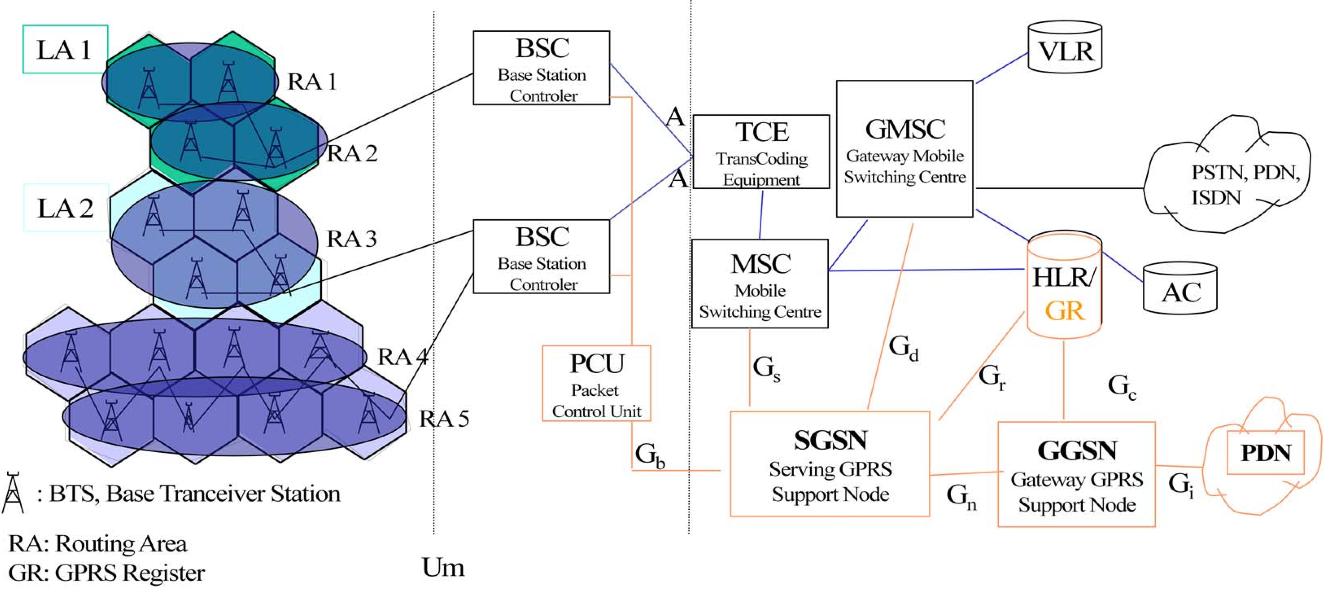
\includegraphics[width = \linewidth]{./Pics/GPRS.png} \\
Diese Grafik zeigt sehr gut, dass das GPRS kein neues Netz ist sondern eine Erweiterung von GSM. Orange eingefärbt sieht man die neuen Element. Man hat nun neben dem Verbindungsorientierten GSM Netz noch ein Paketorierntiertes GPRS Datennetz. Dieses Netz wird ausschliesslich zur Datenübertragung verwendet und kann wegen einer sehr hohen latenzzeit (bis 500ms) auch nicht für VOIP verwendet werden.

\subsubsection{Protocol stack}
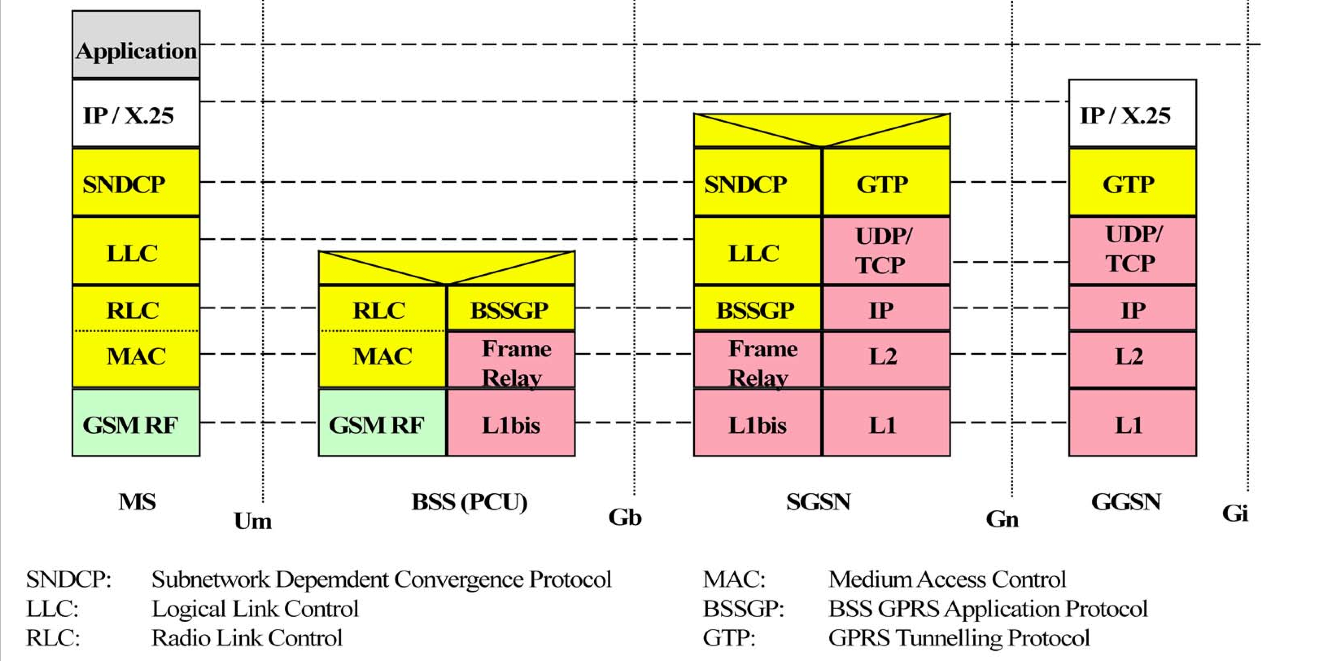
\includegraphics[width = \linewidth]{./Pics/GPRS2.png}

\begin{tabular}{|l|l|l|l|}
\hline
IP & Internet Protocol & X.25 & vorläufer von IP \\
SNDCP & Subnetwork Dependent Convergence Protocol & LLC & Logical Link Control \\
RLC  & Radio Link Control  & MAC & Medium Access Control \\
GSM RF &  Global System for Mobile Communications Radio Frequencies & BSSGP & Base Station System GPRS Protocol \\
GTP & GPRS Tunnelling Protocol & UDP & User Datagram Protocol \\
TCP & Transmission Control Protocol & & \\ 
\hline
\end{tabular}
\subsubsection{GTP}
Das GPRS Tunnelling Protocol baut IP-basierte Verbindungen durch den Backbone auf. Datenpakete werden eingepackt \& unter Benutzung des GTP getunnelt. GTP nutzt unterhalb TCP oder UDP  abhängig von der Nutzeranforderung. Das ganze GPRS Netzwerk basiert auf einem IP Hop, was das Routing im Backbone bei Mobilität vereinfacht.

\subsection{SNDCP - Sub Network Dependent Convergence Protocol}
\begin{itemize}
\item Konvergenz von verschiedenen Protokollen zu einem Data-Link-Protokoll (unterstütz durch das LLC)
\item Multiplext mehrere Verbindungen auf einen Link
\item Header Compression
\item Data Compression
\item Fragmentierung langer Datenpakete
\end{itemize}

\subsection{LLC - Logical Link Control Protocol}

\begin{itemize}
\item Etabliert eine Verbindung zwischen Mobilstation \& SGSN
\item Es kann im bestätigten oder nicht bestätigtem Modus arbeiten
\item Regelung der Datenübertragungswiederholung im bestätigten Modus
\item Unterstützung von point-to-multipoint Adressierung
\end{itemize}

\subsection{RLC - Radio Link Control Protocol}

\begin{itemize}
\item Arbeitet im Bestätigungs-Modus
\item Benutzt den sliding window Mechanismus für die Flusskontrolle
\item Benutzt den Packet Data Treffic Channel
\item Die Bündelung von bis zu 8 PDTCH pro User ist möglich
\item 1 PDTCH hat eine Datenrate von max. 21.4 kbit/s. Daraus ergibt sich die maximale Datenrate von 8 gebündelten PDTCH $\cdot$ 21.4 kbit/s = 171.2 kbit/s
\end{itemize}

\subsection{Logische Kanäle des GPRS}
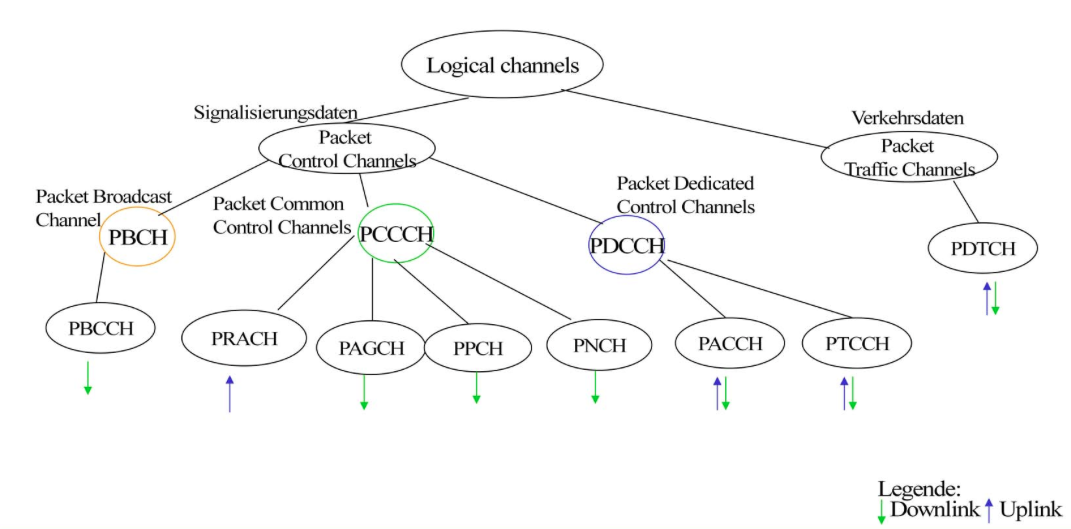
\includegraphics[width = 0.6 \linewidth]{./Pics/GPRSKanaele}

\begin{tabular}{p{0.15 \linewidth} p{0.15 \linewidth} p{0.3 \linewidth} p{0.3 \linewidth}}
\toprule
Logischer Kanal & Richtung & BTS & MS \\
\midrule
PACCH - Packet Associated Control Channel & Downlink and Uplink point to point & Sendet signalisierungsrelevante Information an die MS, z.B. Power Control, acknowledgements. Teilt sich Ressourcen mit dem PDTCH. & Empfängt Signalisierungsdaten und sendet Messreports.\\
\midrule
PAGCH - Packet Access Grant Channel & Downlink point to point & Wird benutzt in der Datenübertragungsaufbauphase zur Ressourcenzuweisung und TA Information (uplink). & Erhält die Ressourcenzuteilung ("timeslots") für den (meist uplink) Datenverkehr zu TA. \\
\midrule
PBCCH - Packet Broadcast Control Channel & Downlink point to Multipoint & Sendet allgemeine Netz/Systeminformation. Ist kein PBCCH alloziert , kann der BCCH verwendet werden. & Hört die Systeminfo ab. Ist PBCCH nicht implementiert, hört die MS den BCCH ab \\
\midrule
PDTCH - Packet Data Traffic Channel & Entweder Uplink oder Downlink Point to point/multipoint nur im DL & Daten werden übermittelt & Daten werden von MS empfangen oder gesendet. \\
\midrule
PNCH - Packet Notification Channel & Downlink point to Multipoint-Multicast & Notification an eine Gruppe von Mobilstationen, wenn multicast traffic ansteht. Wird zur Zuweisung der benötigten Ressourcen ("timeslot") verwendet & Zuweisung der timeslots\\
\midrule
PPCH - Packet Paging Channel & Downlink point to point & Wird hauptsächlich benutzt, um einen downlink Paketdatentransfer einzurichten. Der PPCH kann für Paketservice oder Circuit Switched Services verwendet werden. & Erhält die Ressourcenzuteilung ("timeslots") für den downlink Datenverkehr. \\
\midrule
PRACH - Packet Random Access Channel & Uplink point to point & Ermittelt die Timing Advance info & Benutzt die MS, um einen uplink Transfer zu etablieren \\
\midrule
PTCCH - Packet Timing Advance Control Channel & Entweder uplink oder downlink point to point & Ermittelt TA durch erhalt von Access Burst (erhalt durch UL) Sendet TA an eine Stadtion. & Sendet Access Burst zur BS. Wendet TA an. \\
\bottomrule
\end{tabular}